\documentclass{ctexart}
\usepackage{PhysicalChemistryNote}

\begin{document}\pagestyle{plain}
%
\begin{center}
    \tbf{\Huge Chapter 1 气体}
\end{center}\vspace{15pt}

\indent 欢迎来到物理化学的世界!\footnote{本书的章节导言均由DeepSeek生成.}\\
\indent 在这里,你即将与一群“自由散漫”的气体分子展开一场充满哲学意味的对话.%
是的,它们看似毫无纪律(毕竟连分子间作用力都懒得维持),但正是这些“懒汉”构成了人类理解热力学与物质世界的完美起点.%
如果你曾对着一只气球发呆,疑惑它为何越吹越大却不会爆炸;%
或者试图和17世纪的人们一样因为痴迷热气球旅行而试图弄清楚烧热的气体为什么会带你飞向蓝天,%
那么本章将解答你的(至少是一部分)疑惑.\\
\indent 气体,这个看似“稀薄透明”的章节,实则藏着一部人类与自然法则斗智斗勇的史诗.%
从波义耳在17世纪用简陋的汞柱实验发现压强与体积的反比关系,到焦耳为了测热功当量差点烧穿实验室的桌子,%
科学家们用鲜血(好吧,主要是汞蒸气),汗水和咖啡因,硬生生从混乱的分子运动中提炼出了秩序.\\
\indent 在本章,你将见证%
理想气体如何用一句简洁的$pV=nRT$统治教科书,却在现实中被van der Waals方程无情揭穿"完美人设";%
温度的本质是分子运动的速度快慢,而压强不过是它们对容器壁的集体"拍打抗议".%
当然,我们也会严肃讨论(至少假装严肃):%
为什么研究气体像驯服一群喝醉的蜜蜂?%
为何"理想气体"在现实中(也许)的唯一用途,是让考试题看起来不那么绝望?%
以及,当你在实验室里手抖打翻液氮罐时,气体如何瞬间从"理论模型"变成"职场危机"……\\
\indent 最后,请记住:气体虽轻,但它的故事重若千钧.它是热力学的序章,统计力学的新手村,更是你理解物理化学的入门课.%
毕竟,如果连这群"自由奔放"的分子都搞不定,后面的液体,固体大概会联名要求你再好好学学了.\\
\indent 盖好瓶塞,检查好气密性,调整好气压——我们的分子冒险,现在开始.
\newpage\documentclass{ctexart}
\usepackage{PhysicalChemistryNote}

\begin{document}\pagestyle{plain}
\noindent\tbf{\LARGE 1A 理想气体$^\ast$\footnote{标$\ast$的内容表示你应该在第一次学习物理化学时(或者更应试地说,参加初赛之前)掌握.}}\vspace{15pt}\\
%
\indent 几百年前的人们在艰苦而简陋的实验室里通过日复一日的测定建立了一套定量描述气体的定律.%
这些定律最终都指向我们所熟知的理想气体定律.不过在此之前,我们需要学习如何描述气体.\vspace{12pt}\\
\Section{1A.1 状态函数}
\indent 顾名思义,状态函数是以"状态"为自变量的函数\footnote{我们将在\tbf{2A}中给出更加明确的定义.}.如果两个物体具有相同的状态,那么它们的一些物理性质也应当相同.%
因此,状态函数可以定量的描述系统的状态.我们将在后面的学习中更进一步地了解各种状态函数.\\
\indent 在本章,我们只需知道表征气体系统状态的变量包括物质的量$n$,压强$p$,温度$T$和体积$V$.%
如果气体是由多种物质混合而成的,那么我们还需要各个组分的物质的量.\\
\indent 物质的量和体积都是我们熟知的,在这里我们主要对压强和温度进行简单的讨论.
\begin{definition}[1A.1.1 压力与压强]
    \tbf{压力(compressive force)}是物体间相互挤压而垂直作用在物体表面的一种弹性力,其作用效果用压力除以受力面积表示,称为\tbf{压强(pressure)},用字母$p$表示.\\
    上述名词在不同地方略有不同.在研究气体时,我们提到气体的压力通常就指它的压强,是由于大量气体分子撞击器壁所产生的持续且稳定的力造成的.
\end{definition}
我们所说的器壁并非特指盛装气体的容器.它可以是任何限制气体运动的物体.%
你感受不到大气对你的压力也许只是因为你的身体里也有气体,不是因为你不是器壁.
\begin{definition}[1A.1.2 压力的单位,标准压力]
    压力的SI(国际单位制)单位为帕斯卡(Pa),定义为$1\text{ Pa}=1\text{ N}\cdot\text{m}^{-2}$.\\
    此外,常用的单位有kPa,bar等.我们有
    \[1\text{ bar}=100\text{ kPa}=10^5\text{ Pa}\]
    定义压力$1\text{ bar}$为\tbf{标准压力},记作$p^\ominus$.
\end{definition}
相比于压力,我们对温度的认识也许更粗浅一些.考虑我们感受温度或者温度计测定温度的方式,都是与被测物体直接接触,通过热交换判断物体的冷热程度.%
因此,温度可以被简单地作为当两个物体接触时,热量传递方向的判据:总是从温度高的物体传向温度低的物体.
\begin{definition}[1A.1.3 温度的单位,温标]
    \tbf{温标}是标定温度大小的方式.\\
    我们常用\tbf{摄氏温标}(单位为$\tccentigrade$)或\tbf{热力学温标}(单位为K)描述物体的温度.它们之间有如下换算关系
    \[T/\text{K}=\theta/\tccentigrade+273.15\]
    其中$T$和$\theta$分别表示同一温度在热力学温标和摄氏温标下的温度.
\end{definition}
\begin{hint}
    在\tbf{2A.2}中,我们将基于热力学第零定律对温度和热的定义做更详细的讨论.\\
    在\tbf{1B.1.4}中,我们将基于分子动理论提出第一种温标,即\tbf{理想气体温标}.%
    在\tbf{3D.1.1}中,我们将基于热力学第二定律提出第二种温标,即上面所述的\tbf{热力学温标},%
    并证明热力学温标和理想气体温标实际上是等价的.
\end{hint}\vspace{8pt}
\Section{1A.2 理想气体状态方程}
\Part{状态方程}
\indent 原则上,我们可以用\tbf{1A.1}中提到的四个量$n,p,T,V$表示组分单一的气体的状态.%
然而,大量的实验表明,给定其中的三个量,第四个量也就随之确定了.也就是说,经验告诉我们这四个量之间存在一定的关系.我们把它称作\tbf{状态方程}.
\begin{definition}[1A.2.1 状态方程]
    状态方程是这样的一个方程,它描述了物质的各个状态函数之间存在的等量关系.%
    例如,关于$n,p,T,V$四个状态函数的状态方程具有通式$p=f(n,T,V)$或$V=f(n,p,T)$,等等.
\end{definition}
\Part{描述气体的经验定律和理想气体状态方程}
人们对于气体的研究由来已久,也提出了很多经验定律(如前言所说,多半是为了热气球旅行).你也许在普通化学的学习中已经见过它们,不过我们还是在此加以罗列(虽然,在你掌握理想气体状态方程后,你不记得其中的任何一个也没关系).
\begin{theorem}[1A.2.2 描述气体的经验定律]
    \begin{enumerate}[label=\tbf{\arabic*.}]
        \item \tbf{Boyle$-$Mariotte定律}\\
            定温定量下气体的体积与压力成反比,即
            \[pV=C\]
            其中$C$为常数,下同.
        \item \tbf{Charles$-$Gay-Lussac定律}\\
            定量定压下气体的体积和温度成正比,即
            \[\dfrac VT=C\]
            以及,定量定容下气体的压力和温度成正比,即
            \[\dfrac pT=C\]
        \item \tbf{Avogadro原理}\\
            定温定压下气体的体积和物质的量成正比,即
            \[\dfrac Vn=C\]

    \end{enumerate}
\end{theorem}
\tbf{1A.2.2.1}和\tbf{1A.2.2.2}作为经验定律都是有限制的,它们在$p\to0$时才严格地成立.%
不过,在一般条件下(例如大气压),它们也能很好地符合气体的行为.\\
\indent 对上述几个式子进行适当的变换(尽管并不严谨)即可得到$\dfrac{pV}{nT}=C$.定义式中的常数为气体常数$R$,我们就得到了\tbf{理想气体状态方程}.
\begin{theorem}[1A.2.3 理想气体状态方程]
    当压力趋于$0$时,对所有气体都有状态方程
    \[pV=nRT\]

\end{theorem}
\begin{proof}
    我们刚才说的"并不严谨"是指把\tbf{1A.2.2.2}和\tbf{1A.2.2.3}直接相乘得到
    \begin{equation}
        \dfrac{pV}{nT}=C
    \end{equation}
    尽管这一步看似合理,但是却忽略了各个定律不同的使用范围.Charles定律要求定量定容,而Avogadro原理要求定温定压.(1)的得出自然有不合理之处.\\
    这里,我们采用一种更加严谨的,也更加"数学"的方式进行推导.\\
    对状态方程的一般式
    \begin{equation}
        V=f(n,p,T)
    \end{equation}
    全微分可得
    \begin{equation}
        \di V=\pa{V}{n}{p,T}\di n+\pa{V}{p}{n,T}\di T+\pa{V}{T}{n,p}\di V
    \end{equation}
    根据Avogadro原理,定温定压下气体的体积和物质的量成正比,即$V=C_1n$.于是
    \begin{equation}
        \pa{V}{n}{p,T}=C_1=\dfrac{V}{n}
    \end{equation}
    根据Boyle$-$Mariotte定律,定温定量下气体的体积与压力成反比,即$pV=C_2$,于是
    \begin{equation}
        \pa{V}{p}{n,T}=\dfrac{\p}{\p p}\left(\dfrac{C_2}p\right)=-\dfrac{C_2}{p^2}=-\dfrac{V}{p}
    \end{equation}
    根据Charles$-$Gay-Lussac定律,定量定压下气体的体积和温度成正比,即$V=C_3T$,于是
    \begin{equation}
        \pa{V}{T}{n,p}=C_3=\dfrac{V}{T}
    \end{equation}
    将(4)(5)(6)代入(3)中有
    \begin{equation}
        \di V=\dfrac{V}{n}\di n-\dfrac{V}{p}\di p+\dfrac{V}{T}\di T
    \end{equation}
    移项积分可得
    \begin{equation}
        \ln p+\ln V=\ln T+\ln n+C
    \end{equation}
    即
    \begin{equation}
        \dfrac{pV}{nT}=C'
    \end{equation}
    令积分常数$C'=R$,则有
    \begin{equation}
        pV=nRT
    \end{equation}
    
\end{proof}
\setcounter{equation}{0}
由于实际气体只在$p\to0$时满足理想气体状态方程,因此我们可以对总是满足这方程的气体做一种理想化的定义(尽管它并不存在).
\begin{definition}[1A.2.4]
    在任何压力下都符合\tbf{1A.2.3}的气体称为\tbf{理想气体}.
\end{definition}
\end{document}
\newpage\documentclass{ctexart}
\usepackage{PhysicalChemistryNote}

\begin{document}\pagestyle{plain}
\noindent\tbf{\LARGE 1B 气体分子动理论}\vspace{15pt}\\
%
\indent 据说,从前有个农民,他养了一些鸡,但是它们不下蛋.于是他去找物理学家求救.%
这个物理学家便做了些计算,然后说:"我有个办法,不过只适用于真空中的球形鸡."\\
\indent 虽然这个笑话讽刺了物理学家们做的研究似乎总是不太切实际(恕我直言,现代化学也有相当一部分是这样),但是所有的理论总是建立在一个又一个理想化的假设上的.%
当我们知道了这些假设和它们的推论,也就离描述真实的世界又近了一步.毕竟,真空中的球形鸡也是一种鸡.\vspace{12pt}\\
\Section{1B.1 气体分子动理论的基本公式}
\Part{气体分子动理论的基本方程}
\indent 我们从气体分子运动的微观模型开始本节.
\begin{theorem}[1B.1.1 气体分子运动的微观模型]
    (理想)气体分子运动的微观模型可表述为:
    \begin{enumerate}[label=\tbf{\arabic*.}]
        \item 气体是大量分子的集合体.相较于气体分子之间的距离和所占据的体积,%
            其本身的体积是很小而可以忽略不计的.因此,可以把气体分子当作质点处理.
        \item 气体分子总是做无规则的运动,均匀分布在容器中.
        \item 分子之间的碰撞或分子与容器壁的碰撞是完全弹性的.
    \end{enumerate}
\end{theorem}
应当思考的是,一定量的气体在一定体积下具有恒定的压强.%
从微观角度解释,这一压强来源于大量气体分子均匀地碰撞容器壁而产生.%
因此,压强和体积这两个宏观物理量应当与气体分子的微观性质(例如运动速度,质量,数目等等)相关联.%
下面我们从上述假设和一些基本的物理知识推导联系上述宏观量和微观量的\tbf{气体分子动理论的基本方程}.
\begin{derivation}
    为了简单考虑,我们不妨设容器为一个边长为$l$的正方体.一个质量为$m$的粒子$X_i$以$v_i$的速度沿$x$轴撞击某一壁.\\
    根据\tbf{1B.1.1.3}可知该分子与容器壁的碰撞是完全弹性的,于是该过程的动量变化为
    \[\Delta p=mv_{x,i}-\left(-mv_{x,i}\right)=2mv_{x,i}\]
    其中$v_{x,i}$为$X_i$沿$x$方向的速度分量.$X_i$每隔$\dfrac{2l}{v_{x,l}}$的时间便撞击一次该壁,于是此面受的力为
    \[F_{x,i}=\dfrac{\Delta p}{\Delta t}=\dfrac{2mv_{x,i}}{\frac{2l}{v_{x,i}}}=\dfrac{mv_{x,i}^2}{l}\]
    考虑容器内的所有粒子,假定它们质量相同,总数目为$N$,则有
    \[\sum F_x=\dfrac{\displaystyle \sum_{i=1}^{N}mv_{x,i}^2}{l}=\dfrac ml\sum_{i=1}^{N}v_{x,i}^2\]
    令$\displaystyle \overline{v_x^2}=\dfrac{1}{N}\sum_{i=1}^{N}v_{x,i}^2$,$F_x=\dfrac{mN\overline{v_x^2}}{l}$,其中$F_x$即为所有分子对$x$方向某侧器壁的作用力.同理可得
    \[F_y=\dfrac{mN\overline{v_y^2}}{l}\ \ \ \ \ F_z=\dfrac{mN\overline{v_z^2}}{l}\]
    又因为$v_{x,i}^2+v_{y,i}^2+v_{z,i}^2=v_i^2$,于是可以定义
    \[\overline{v^2}=\dfrac{1}{N}\sum_{i=1}^{N}v_i^2=\overline{v_x^2}+\overline{v_y^2}+\overline{v_z^2}\]
    根据\tbf{1B.1.1.2}和正方体的对称性可知,各个方向上器壁的受力应当相同,于是$F_x=F_y=F_z$,从而
    \[\overline{v_x^2}=\overline{v_y^2}=\overline{v_z^2}\ \ \ \ \ \overline{v^2}=3\overline{v_x^2}\]
    每个面受到的压强$p$为
    \[p=\dfrac{F}{S}=\dfrac{\frac{mN\overline{v_x^2}}{l}}{l^2}=\dfrac{mN\overline{v_x^2}}{l^3}=\dfrac{mN\overline{v^2}}{3V}\]
    移项即可得
    \[pV=\dfrac13mN\overline{v^2}\]
    如果令$u=\sqrt{\dfrac1N\displaystyle\sum_{i=1}^{N}v_i^2}$,称为\tbf{均方根速率},则有
    \[pV=\dfrac13mNu^2\]

\end{derivation}
我们就得到了联系宏观量和微观量的一个方程.
\begin{theorem}[1B.1.2 气体分子动理论的基本方程]
    设气体体积为$V$,压强为$p$,气体分子质量为$m$,数目为$N$,均方根速率为$u$,则有
    \[pV=\dfrac13mNu^2\]

\end{theorem}
\Part{压强和温度的统计学意义}
\indent 由\tbf{1B.1.2},我们可以得到压强$p$的统计学意义.在上述推导中,压强实际上就是大量分子撞击器壁产生的总结果.
\begin{theorem}[1B.1.3 压强的统计学意义]
    大量气体分子撞击器壁,总体来说器壁受到的作用力(压力)具有持续性,稳定性.在宏观上这就表现为压强.
\end{theorem}
那么温度究竟是什么呢?我们在\tbf{1A}中对温度做过一个粗浅的定义,用于衡量两个物体接触时热量的传递方向.%
对于两个温度不同的气体(不妨假定为A和B),假定它们的能量仅来源于其动能,那么交换能量的方式就是通过碰撞而互相传递能量.%
在宏观上就表现为平均动能\footnote{这里指的是平动能,即分子整体移动的动能,而有别于转动能.}.高的气体分子向平动能低的气体分子传递能量.%
因此,如果它们的温度不同,就应当具有平动能上的的区别.否则,如果平动能相同,那么宏观上两种气体没有能量传递,也就不应当具有温度的差别.\\
\indent 因此,可以认为平动能$\overline{E_t}=\dfrac12u^2$与温度具有正相关性,平动能越高则气体温度越高,向别的物体传热的能力就越强.%
一种直接而合理的想法是将平动能直接称为温度,不过为了和现行的温度的尺度相符,我们可以添加一个比例系数,即
\[\dfrac12mu^2=\dfrac{3}{2}k_\text BT\]
这里的$k_\text B$即Boltzmann常数,而$\dfrac32$则是方便计算而引入的系数(我们马上就会看到这样写的合理性).这就是基于分子动理论的温度的定义.
\begin{definition}[1B.1.4 理想气体温标]
    理想气体的温度$T$被定义为
    \[\dfrac12mu^2=\dfrac32k_\text BT\]
    其中$\dfrac12mu^2$是气体分子的平均平动能.
\end{definition}
基于这样的温度的定义,我们不难可以得到
\[pV=\dfrac13Nmu^2=Nk_\text BT=nRT\]
如此,你就从气体分子动理论得到了理想气体状态方程.基于这个式子可以得到
\[u=\sqrt{\dfrac{3k_\text BT}{m}}\]
这是一个比较重要的式子,在推导Maxwell速率分布时将要用到.
\begin{hint}
    我们将在\tbf{Chapter 3}中给出温度的另一种定义,即热力学温标,并且说明两种定义的等价性.
\end{hint}\vspace{8pt}
\Section{1B.2 分子运动的速率分布}
\Part{Maxwell速率分布的推导}
\indent 气体包含数量众多的分子.它们在容器内每时每刻都在互相碰撞,其速度都在发生变化.那么,是否有一种方法能总体地描述气体分子运动速率呢?%
我们将从简单的概率论出发推导分子运动的速率的分布情况.\\
\indent 我们首先需要知道一些概率论的知识.当随机变量是离散的时候,我们都知道它的的每一个取值都对应一个大于等于0的概率值.%
例如,均匀的六面骰子掷出1到6中任意一点的概率均为$\frac16$.\\
\indent 然而,当随机变量是连续的时候,我们不再能逐一例举每一个随机变量,而且很显然的一个结论是随机变量的每一个取值的概率都是0.%
例如,在区间$(0,1)$上任意取实数,取到某个特定的实数的概率都是$0$(你可以粗略地理解为$\frac{1}{\infty}$).%
这时,真正有意义的是随机变量落在某一个区间的概率,例如你所取的实数落在区间$\left(0,\frac12\right)$内的概率(直观的)为$\frac12$.
\begin{definition}[1B.2.1 连续随机变量的概率密度函数]
    对于随机变量$x$,我们假定一个概率函数$P(x)$,使得对于某个特定的取值$x_0$,随机变量落在一个无穷小区间$(x_0,x_0+\di x)$内的概率(这当然也是一个无穷小量)满足
    \[P\left(x_0<x<x_0+\di x\right)=\di P(x_0)\]
    如果要求$x$落在区间$(a,b)$内的概率,应当进行积分
    \[P(a<x<b)=\int_a^b\di P(x)\]
    将$\di P(x)$写成$f(x)\di x$,就有
    \[P(a<x<b)=\int_a^bf(x)\dx\]
    我们将这样的函数$f(x)$称作随机变量$x$的\tbf{概率密度函数}.\\
    对于某个特定的$x_0$,$f\left(x_0\right)\dx$就等于$x\in\left(x_0,x_0+\dx\right)$的概率.\\
    概率密度函数需要满足\tbf{归一化}条件.如果$x$的所有可能的取值范围为$(A,B)$,那么我们有
    \[\int_A^Bf(x)\dx=1\]
    这代表$x$落在$(A,B)$内的概率是$1$.
\end{definition}
类似地,分子速率也是一个连续随机函数.我们可以类似地得到分子速率分布函数的定义.
\begin{definition}[1B.2.2 分子速率分布函数]
    在一定温度$T$下,某个气体分子的运动速率$v$是一个连续随机变量.如果关于速率$v$的函数$f(v)$满足对任意的$0<v_a<v_b$都有
    \[P\left(v_a<v<v_b\right)=\int_{v_a}^{v_b}f(v)\di v\]\
    成立,则称$f(v)$是该温度下气体的\tbf{分子速率分布函数}.
\end{definition}
于是,只要我们知道了$f(v)$的具体形式,就能研究分子处于任意一个速率范围内的概率,进而获知气体分子的速率分布.下面我们着手推导$f(v)$.
\begin{derivation}
    设分子的速率为$v$,其速度在空间直角坐标系上可以分解为$v_x,v_y,v_z$.\\
    以$v_x,v_y,v_z$为轴建立一个三维空间.这样,每个分子都可以根据其在三个方向上的速度(含正负)对应到这空间中的一个点.\\
    先考虑$v_x$方向.假定分子总数为$N$,速率处于$\left(v_x,v_x+\di v_x\right)$上的分子数目为$\di N_{v_x}$.这样,分子的$x$方向上速率处于该区间内的概率为$\dfrac{\di N_{v_x}}{N}$.\\
    分子在$x$方向上的速率当然也是连续随机变量,设其概率密度函数为$f_x\left(v_x\right)$.根据\tbf{1B.2.1}可知
    \begin{equation}
        \dfrac{\di N_{v_x}}{N}=f_x\left(v_x\right)\di v_x
    \end{equation}
    类似地,在$y$方向和$z$方向上有
    \begin{equation}
        \dfrac{\di N_{v_y}}{N}=f_y\left(v_y\right)\di v_y\ \ \ \ \ \dfrac{\di N_{v_z}}{N}=f_z\left(v_z\right)\di v_z
    \end{equation}
    根据气体分子运动的特性,我们认为分子在总体上并没有倾向于向任何方向运动(即"没有择优方向"),即速度的分布是各向同性的.%
    于是,我们有理由认为各个方向上的速率分布函数$f_x,f_y,f_z$具有相同的形式,记为$f$.\\
    同样地,我们可以假设各个方向上的速度是独立的.直观地想,分子在某个方向上的速率应当不会影响它在与该方向垂直方向上的速率.\\
    几件独立事件同时发生的概率应当等于它们各自发生的概率之积,%
    于是,在三个方向上的运动速率分别处于$\left(v_x,v_x+\di v_x\right)$,$\left(v_y,v_y+\di v_y\right)$和$\left(v_z,v_z+\di v_z\right)$中的分子的数目$\di N_{v_x,v_y,v_z}$为
    \begin{equation}
        \di N_{v_x,v_y,v_z}=Nf\left(v_x\right)f\left(v_y\right)f\left(v_z\right)\di v_x\di v_y\di v_z
    \end{equation}
    这个区域的体积为$\di V=\di v_x\di v_y\di v_z$.既然我们知道这区域内的分子数目和体积,就可以定义一个密度函数$\rho\left(v_x,v_y,v_z\right)$(注意这里的$\rho$不是概率密度函数,$\dfrac{\rho}{N}$才是),使得
    \begin{equation}
        \rho\left(v_x,v_y,v_z\right)=\dfrac{\di N_{v_x,v_y,v_z}}{\di V}=Nf\left(v_x\right)f\left(v_y\right)f\left(v_z\right)
    \end{equation}
    对$\rho$做偏微分有
    \begin{equation}
        \begin{aligned}
            \di\rho
        &= \left(\dfrac{\p\rho}{\p v_x}\right)\di v_x+\left(\dfrac{\p\rho}{\p v_y}\right)\di v_y+\left(\dfrac{\p\rho}{\p v_z}\right)\di v_z \\
        &= Nf'\left(v_x\right)f\left(v_y\right)f\left(v_z\right)\di v_x+Nf\left(v_x\right)f'\left(v_y\right)f\left(v_z\right)\di v_y+Nf\left(v_x\right)f\left(v_y\right)f'\left(v_z\right)\di v_z
        \end{aligned}
    \end{equation}
    仍然由于速度具有各向同性,因此指定速率为$v$时,只要满足$v_x^2+v_y^2+v_z^2=v^2$,$\rho\left(v_x,v_y,v_z\right)$的取值就应相同.%
    于是在这个球壳上,有$\di\rho=0$,即$\dfrac{\di\rho}{\rho}=0$.于是
    \begin{equation}
        \left\{\begin{array}{l}
            \dfrac{f'\left(v_x\right)}{f\left(v_x\right)}\di v_x+\dfrac{f'\left(v_y\right)}{f\left(v_y\right)}\di v_y+\dfrac{f'\left(v_z\right)}{f\left(v_z\right)}\di v_z=0 \\
            v_x\di v_x+v_y\di v_y+v_z\di v_z=0
        \end{array}\right.
    \end{equation}
    后者是对球面方程微分得到的,决定了$\di v_x,\di v_y,\di v_z$之间满足的关系.前者是速率分布的各向同性决定的$\rho$在球面上的取值不变而得到的.%
    现在,我们要在这两个限制条件下求解$f$的表达式.考虑Lagrange乘数法,将第二个方程乘以参数$\lambda$后与第一个方程相加可得
    \begin{equation}
        \left(\dfrac{f'\left(v_x\right)}{f\left(v_x\right)}+\lambda v_x\right)\di v_x
        +\left(\dfrac{f'\left(v_y\right)}{f\left(v_y\right)}+\lambda v_y\right)\di v_y
        +\left(\dfrac{f'\left(v_z\right)}{f\left(v_z\right)}+\lambda v_z\right)\di v_z=0
    \end{equation}
    选定$\lambda$使得
    \begin{equation}
        \dfrac{f'\left(v_x\right)}{f\left(v_x\right)}+\lambda v_x=0
    \end{equation}
    则上式变为
    \begin{equation}
        \left(\dfrac{f'\left(v_y\right)}{f\left(v_y\right)}+\lambda v_y\right)\di v_y
        +\left(\dfrac{f'\left(v_z\right)}{f\left(v_z\right)}+\lambda v_z\right)\di v_z=0
    \end{equation}
    现在,$\di v_y$和$\di v_z$不再有限定关系(无论这两者如何变化,我们都可以根据(6)求出$\di v_x$后使得约束条件成立).令$\di v_y=0$可得
    \begin{equation}
        \dfrac{f'\left(v_z\right)}{f\left(v_z\right)}+\lambda v_z=0
    \end{equation}
    同理令$\di v_z=0$可得
    \begin{equation}
        \dfrac{f'\left(v_y\right)}{f\left(v_y\right)}+\lambda v_y=0
    \end{equation}
    于是我们得到了三个形式相同的微分方程.以(8)为例,变形可得
    \[\dfrac{\di f\left(v_x\right)}{f\left(v_x\right)}=-\lambda v_x\di v_x\]
    两边积分可得
    \[\ln f\left(v_x\right)=-\dfrac12\lambda v_x^2+\ln\alpha\]
    式中$\alpha$为积分常数.令$\beta^2=\dfrac12\lambda$,并取指数有
    \begin{equation}
        f\left(v_x\right)=\alpha\e^{-\beta^2v_x^2}
    \end{equation}
    同理
    \begin{equation}
        f\left(v_y\right)=\alpha\e^{-\beta^2v_y^2}
    \end{equation}
    \begin{equation}
        f\left(v_z\right)=\alpha\e^{-\beta^2v_z^2}
    \end{equation}
    将(12)(13)(14)代入(4)中可得
    \begin{equation}
        \rho\left(v_x,v_y,v_z\right)=N\alpha^3\exp\left(-\beta^2\left(v_x^2+v_y^2+v_z^2\right)\right)=N\alpha^3\exp\left(-\beta^2v^2\right)
    \end{equation}
    于是密度函数是以$v$为自变量的函数.\\
    考虑速度落在$(v,v+\di v)$区间上的分子,这是一个球壳层,其体积为$\di V=4\pi v^2\di v$.在这个球壳层内,分子分布的密度$\rho$近似相等,于是在这个球壳上分布的分子数目$\di N_v$为
    \begin{equation}
        \di N_v=\rho(v)\di V=N\alpha^3\exp\left(-\beta^2v^2\right)\cdot4\pi v^2\di v
    \end{equation}
    由于分子速率一定处于$(0,+\infty)$上,于是
    \begin{equation}
        \int_{0}^{+\infty}\di N_v=\int_{0}^{+\infty}N\alpha^3\exp\left(-\beta^2v^2\right)\cdot4\pi v^2\di v=N
    \end{equation}
    化简可得
    \[4\pi\alpha^3\int_0^{+\infty}v^2\exp\left(-\beta^2v^2\right)\di v=1\]
    查阅积分表可得
    \[\int_0^{+\infty}v^2\exp\left(-\beta^2v^2\right)\di v=\dfrac{\sqrt\pi}{4\beta^3}\]
    代入上式可得
    \begin{equation}
        \sqrt\pi\alpha=\beta
    \end{equation}
    又因为均方根速率
    \begin{equation}
        u=\sqrt{\int_{0}^{+\infty}v^2F(v)\di v}=\sqrt{\dfrac{3k_\text BT}{m}}
    \end{equation}
    于是
    \[\dfrac{3k_\text BT}{m}=\dfrac{4\beta^3}{\sqrt\pi}\int_0^{+\infty}v^4\exp\left(-\beta^2v^2\right)\di v\]
    查阅积分表可得
    \[\int_0^{+\infty}v^4\exp\left(-\beta^2v^2\right)\di v=\dfrac{3\sqrt\pi}{8\beta^5}\]
    于是
    \begin{equation}
        \dfrac{3k_\text BT}{m}=\dfrac{3}{2\beta^2}
    \end{equation}
    根据(18)与(20)可得
    \[\alpha=\sqrt{\dfrac{m}{2\pi k_\text BT}}\ \ \ \ \ \beta=\sqrt{\dfrac{m}{2k_\text BT}}\]
    代入(16)可得
    \begin{equation}
        \di N_v=\dfrac{4N}{\sqrt\pi}\left(\dfrac{m}{2k_\text BT}\right)^{\frac32}v^2\text{exp}\left(-\dfrac{mv^2}{2k_\text BT}\right)\di v
    \end{equation}
    根据$\di N_v$的定义,$\dfrac{\di N_v}{N}$表示气体速率在$(v,v+\di v)$内的概率,因而根据\tbf{1B.2.1}可知
    \begin{equation}
        \dfrac{\di N_v}{N}=f(v)\di v
    \end{equation}
    其中$f(v)$为气体的速率分布函数.将(21)代入(22)有
    \[f(v)=\dfrac{4}{\sqrt\pi}\left(\dfrac{m}{2k_\text BT}\right)^{\frac32}v^2\text{exp}\left(-\dfrac{mv^2}{2k_\text BT}\right)\]
    这就是Maxwell速率分布函数.
\end{derivation}\setcounter{equation}{0}
总结我们的推导过程,大致按照
\begin{enumerate}[label=\tbf{\arabic*.}]
    \item 写出各个方向上的速率分布函数$f\left(v_x\right)$,$f\left(v_y\right)$,$f\left(v_z\right)$.
    \item 用运动的各向同性写出在速率空间内的密度函数$\rho\left(v_x,v_y,v_z\right)$.
    \item 考虑到$\rho\left(v_x,v_y,v_z\right)$在球壳上的取值不变,写出关于$f$的微分方程.
    \item 求解$f$和$\rho$的含待定参量$\alpha,\beta$的形式.
    \item 根据概率密度函数的归一化性质和分子的均方根速率求得待定的参量$\alpha,\beta$.
    \item 得出速率分布函数.
\end{enumerate}
的过程进行推导.这样就得到了Maxwell速率分布.
\begin{theorem}[1B.2.2 Maxwell速率分布]
    气体分子运动的速率函数$f(v)$具有如下形式
    \[f(v)=\dfrac{4}{\sqrt\pi}\left(\dfrac{m}{2k_\text BT}\right)^{\frac32}v^2\text{exp}\left(-\dfrac{mv^2}{2k_\text BT}\right)\]

\end{theorem}
下面绘制了不同温度和分子质量下的Maxwell速率分布的图像,以供你理解这一分布的性质.%
可以看到,分子质量越大,温度越低,速率分布的越集中.
\begin{figure}[H]
    \centering\documentclass{standalone}
\usepackage{PhysicalChemistryNote}
\begin{document}
\begin{tikzpicture}
    \begin{axis}[
        width = 12cm,
        height = 8cm,
        legend pos = north east,
        xlabel = {速率 $v/\left(\mathrm{m}\cdot\mathrm{s}^{-1}\right)$},
        ylabel = {概率密度 $f(v)/10^{-3}$},
        axis lines = left,
        ymax = 3.5,
        domain = 0:3000,
        samples = 400
    ]
    \addplot [thick, blue] {(4 / sqrt(pi)) *0.0000133* x^2 * exp(-0.0000056*x^2)};
    \addplot [thick, red] {(4 / sqrt(pi)) *0.000069* x^2 * exp(-0.0000168*x^2)};
    \addplot [thick, yellow] {(4 / sqrt(pi)) *0.000000254* x^2 * exp(-0.0000004*x^2)};
    \addplot [thick, cyan] {(4 / sqrt(pi)) *0.00000132* x^2 * exp(-0.0000012*x^2)};
    \legend {$\text{N}_2\left(300\text{K}\right)$,
        $\text{N}_2\left(100\text{K}\right)$,
        $\text{H}_2\left(300\text{K}\right)$,
        $\text{H}_2\left(100\text{K}\right)$,}
    \end{axis}
\end{tikzpicture}
\end{document}
\end{figure}
\Part{描述分子速率分布的三个特征量}
\indent 不难发现,上图的每条曲线都有一个最高点,表示具有该速度的分子所占比例最大.于是可以做如下定义.
\begin{definition}[1B.2.3 最概然速率]
    分子的\tbf{最概然速率}$v_m$是气体分子在一定条件下最有可能具有的速率,对应速率分布函数$f(v)$取到最大值时$v$的取值.
\end{definition}
我们可以尝试对$v_m$的具体值进行推导.
\begin{derivation}
    $f(v)$图像的最高点满足
    \[\dfrac{\di f(v)}{\di v}=0\]
    于是
    \[\dfrac{\di}{\di v}\left(v^2\exp\left(-\dfrac{mv^2}{2k_{\text BT}}\right)\right)=0\]
    化简可得
    \[\left(2v-\dfrac{mv^3}{k_{\text BT}}\right)\exp\left(-\dfrac{mv^2}{2k_{\text BT}}\right)=0\]
    由此解得
    \[v=\sqrt{\dfrac{2k_\text BT}{m}}=\sqrt{\dfrac{2RT}{M}}\]

\end{derivation}
由此可见,分子的最概然速率与温度的平方根成正比,与摩尔质量的平方根成反比,这也符合我们对图像的观察.\\
\indent 除了最概然速率之外,还有一个值得考量的统计量,即所有分子的速率的数学平均值.
\begin{definition}[1B.2.4 数学平均速率]
    分子的\tbf{数学平均速率}$v_a$是所有分子速率的数学平均值.
\end{definition}
同样地,我们也可以计算$v_a$的具体值.
\begin{derivation}
    考虑所有$N$个分子,处于速率$v$的分子有$\di N_v$个,将它们求和(对无穷小量的求和实际上就是积分运算)有
    \[v_a=\dfrac{\displaystyle\sum v\cdot\di N_v}{N}=\dfrac1N\int_{0}^{+\infty}v\di N_v
    =\int_0^{+\infty}\dfrac{4}{\sqrt\pi}\left(\dfrac{m}{2k_\text BT}\right)^{\frac32}v^3\text{exp}\left(-\dfrac{mv^2}{2k_\text BT}\right)\di v\]
    做代换$x=\dfrac{mv^2}{2k_\text BT}$,则上式可以写作
    \[v_a=\sqrt{\dfrac{8k_\text BT}{\pi m}}\int_{0}^{+\infty}x\e^{-x}\di x\]
    查阅积分表可得
    \[\int_{0}^{+\infty}x\e^{-x}\di x=1\]
    于是
    \[v_a=\sqrt{\dfrac{8k_\text BT}{\pi m}}\]

\end{derivation}
至此,我们得到了关于分子运动速率的三个统计量:均方根速率$u$,最概然速率$v_m$和数学平均速率$v_a$.它们之间的比例关系如下
\[v_m:v_a:u=\sqrt2:\sqrt{\dfrac8\pi}:\sqrt3\]
\Section{1B.3 分子平动能的分布}
\indent 从Maxwell分布很容易就能推出分子能量(这里指的就是平动能)的分布.
\begin{derivation}
    各分子的平动能为$E=\dfrac12mv^2$,于是
    \[\di E=mv\di v\]
    代入\tbf{1B.2.2}有
    \[f(E)=\dfrac{2}{\sqrt\pi}\left(\dfrac{1}{k_\text BT}\right)^{\frac32}\sqrt{E}\exp\left(-\dfrac{E}{k_\text BT}\right)\]
    其实就是把$f(v)$改写成$E$的函数以得到关于能量的分布.
\end{derivation}
\begin{theorem}[1B.3.1 三维空间中的能量分布函数]
    分子平动能在三维空间中的\tbf{能量分布函数}$f(E)$为
    \[f(E)=\dfrac{2}{\sqrt\pi}\left(\dfrac{1}{k_\text BT}\right)^{\frac32}\sqrt{E}\exp\left(-\dfrac{E}{k_\text BT}\right)\]
    对于任意的$0<E_1<E_2$,分子能量$E$满足$E_1<E<E_2$的概率为
    \[P\left(E_1<E<E_2\right)=\int_{E_1}^{E_2}f(E)\di E\]

\end{theorem}
我们还可以考虑所有分子中能量大于$E_0$的分子的数目$N_{E_0\to\infty}$(这在化学反应动力学的研究中非常重要).根据\tbf{1B.3.1}就有
\[\dfrac{N_{E_0\to\infty}}{N}=P\left(E_0<E\right)=\int_{E_0}^{+\infty}f(E)\di E\]
用分部积分法对上面的积分做展开,可得
\[\dfrac{N_{E_0\to\infty}}{N}=\dfrac{2}{\sqrt\pi}\sqrt{\dfrac{E_0}{k_\text BT}}\exp\left(\dfrac{E_0}{k_\text BT}\right)\left[1+\left(\dfrac{k_\text BT}{2E_0}\right)-\left(\dfrac{k_\text BT}{2E_0}\right)^2+3\left(\dfrac{k_\text BT}{2E_0}\right)^3-\cdots\right]\]
一般情况下$E_0\gg k_\text BT$,因此求和项可以只保留第一项.于是我们有
\begin{theorem}[1B.3.2 大于某个能量值的分子数目]
    气体分子能量大于某个定值$E_0$的概率为
    \[P_{E_0\to\infty}=\dfrac{N_{E_0\to\infty}}{N}=\dfrac{2}{\sqrt\pi}\sqrt{\dfrac{E_0}{k_\text BT}}\exp\left(\dfrac{E_0}{k_\text BT}\right)\]

\end{theorem}
通常在物理化学中,我们只需用到能量分布的近似公式,这是通过二维空间中的Maxwell速率分布推出的.%
在我们学习推导三维空间中的情况后,也许此时你可以先合上书,在草稿纸上自己演算一遍.
\begin{derivation}
    设分子速率为$v$,其速度在平面直角坐标系上可以分解为$v_x,v_y$.\\
    同样地,建立一个二维的速度空间将每个分子对应到其上的一点.\\
    考虑$x$方向和$y$方向的速率分布函数$f_x\left(v_x\right)$和$f_y\left(v_y\right)$.与三维空间相同地,我们有
    \[f\left(v_x\right)=\alpha\e^{-\beta^2v_x^2}\]
    \[f\left(v_y\right)=\alpha\e^{-\beta^2v_y^2}\]
    于是概率密度函数
    \[\rho\left(v_x,v_y\right)=Nf\left(v_x\right)f\left(v_y\right)
    =\dfrac{Nm}{2\pi k_\text B T}\exp\left(-\dfrac{v^2}{2k_\text BT}\right)\]
    做极坐标变换,即$v_x=v\cos\theta,v_y=v\sin\theta$,则$\di v_x\di v_y=v\di v\di\theta$.%
    考虑到所有速率为$v$的分子,运动方向介于$0$到$2\pi$之间,于是
    \[\di N_v=\int_{v_x^2+v_y^2=v^2}\rho\di v_x\di v_y=\int_{0}^{2\pi}\rho v\di v\di \theta=2\pi\rho\di v\]
    从而速率分布函数
    \[f(v)=\dfrac{\di N_v}{\di v}=2\pi\rho=\left(\dfrac{Nm}{k_\text BT}\right)v\exp\left(-\dfrac{v^2}{2k_\text BT}\right)\]
    与三维空间中同理可以推出
    \[f(E)=\dfrac{N}{k_\text BT}\exp\left(-\dfrac{E}{k_\text BT}\right)\]
    进行无穷积分可得
    \[\dfrac{N_{E_0\to\infty}}{N}=\int_{E_0}^{+\infty}f(E)\di E=\exp\left(-\dfrac{E_0}{k_\text BT}\right)\]
    
\end{derivation}
这就是我们更常用的能量分布公式.事实上,这正是Boltzmann分布的结果.
\begin{theorem}[1B.3.3 能量分布的近似公式]
    在二维空间中,气体分子的能量分布函数
    \[f(E)=\dfrac{N}{k_\text BT}\exp\left(-\dfrac{E}{k_\text BT}\right)\]
    气体分子能量大于某个定值$E_0$的概率为
    \[P_{E_0\to\infty}=\dfrac{N_{E_0\to\infty}}{N}=\exp\left(-\dfrac{E_0}{k_\text BT}\right)\]
    这一结论在能量分布的推导中更加常用.
\end{theorem}
\vspace{8pt}
\Section{\Large 1B.4 分子的碰撞频率,平均自由程与隙流}
\Part{分子的互碰频率与平均自由程}
\indent 分子以很高的速度做无规则运动,每时每刻都在发生大量的碰撞.研究气体分子的碰撞过程对于了解气体的扩散,热传导等现象具有重要的意义.
\begin{definition}[1B.4.1 自由程与平均自由程]
    分子在两次连续碰撞之间所经过的路程称为\tbf{自由程},记为$l$.\\
    自由程在无规则地不断地改变着,其平均值称为\tbf{平均自由程},记为$\overline{l}$.
\end{definition}
我们知道,分子之间的碰撞实际上是分子靠近后相斥而使它们又互相远离的过程.为了更方便地讨论这一过程,我们定义\tbf{有效直径}.
\begin{definition}[1B.4.2 有效直径]
    分子碰撞时,两个分子的质心所能达到的最短距离称为\tbf{有效直径},记为$d$.
\end{definition}
下面我们着手推导互碰频率与平均自由程.
\begin{derivation}
    设某个分子$X$的半径为$r$,平均速率为$v_a$,在时间$t$内与其它分子碰撞的次数为$z'$,那么显然有
    \begin{equation}
        \overline{l}=\dfrac{v_at}{z'}
    \end{equation}
    我们假定在体积$V$内均匀分布着$N$个分子.首先,假设其它分子都是静止的,仅考虑$X$分子.%
    它在这段时间走过的路程为$v_at$.我们要计算有多少分子会与之发生碰撞,就要考虑有多少分子会落在与$X$的质心距离小于$d=2r$的范围$D_X$内.\\
    换一个角度思考这个问题,我们只需知道区域$D_X$在这段时间扫过的体积和单位体积内的分子数$n$,就可以知道与之发生碰撞的分子总数.\\
    显然,$D_X$是一个以$X$为球心,半径为$d$的球.由于我们假设分子体积忽略不计,那么$d$相对于$v_at$应当很小.于是,这个球扫过的体积可以近似为多段圆柱(这是因为$X$由于碰撞而多次改变方向)的体积.%
    这些圆柱的总长度为$v_at$,圆柱的半径为$d$,因此
    \begin{equation}
        V_X=\pi d^2v_at
    \end{equation}
    又因为单位体积内的分子数目为
    \begin{equation}
        n=\dfrac{N}{V}
    \end{equation}
    于是与$X$发生碰撞的分子总数(实际上就是碰撞次数$z'$)
    \begin{equation}
        z'=n\pi d^2v_at
    \end{equation}
    然后再考虑每个分子都在运动的情况.这时,应当用平均相对速率$v_r$代替上面式子中的$v_a$.\\
    考虑两个分子$X,Y$碰撞时速度(不妨记为$\overrightarrow{v_X},\overrightarrow{v_Y}$)的夹角为$\theta$,它们的相对速率$v_r$应当为
    \[v_r=\left|\overrightarrow{v_X}-\overrightarrow{v_Y}\right|
    =\sqrt{\left|\overrightarrow{v_X}-\overrightarrow{v_Y}\right|^2}
    =\sqrt{\left|\overrightarrow{v_X}\right|^2+\left|\overrightarrow{v_Y}\right|^2-2\left|\overrightarrow{v_X}\right|\left|\overrightarrow{v_X}\right|\cos\theta}\]
    先代入所有分子的平均速率$v_a$,即$\left|\overrightarrow{v_X}\right|=\left|\overrightarrow{v_Y}\right|=v_a$,则有
    \[v_r=v_a\sqrt{2\left(1-\cos\theta\right)}\]
    $\theta$应在$[0,\pi]$上均匀分布,则$\cos\theta$应对称地取遍$[-1,1]$上的值.于是$(1-\cos\theta)$的均值为$1$,于是
    \begin{equation}
        v_r=\sqrt{2}v_a
    \end{equation}
    将(5)代入(4)可得
    \begin{equation}
        z'=\sqrt2v_a\pi d^2nt
    \end{equation}
    于是平均自由程
    \begin{equation}
        \overline{l}=\dfrac{v_at}{z'}=\dfrac{1}{\sqrt2\pi d^2n}
    \end{equation}
    现在,考虑所有$N$个分子,每个分子在时间$t$内发生碰撞的次数均为$z'$.又因为每次碰撞都是两个分子参与的,因此实际次数应是上面计数方法所得的一半.这样,在单位体积内的碰撞频率
    \begin{equation}
        \nu=\dfrac{Nz'}{2Vt}=\dfrac{\pi d^2n^2v_a}{\sqrt2}
    \end{equation}
    将$v_a=\sqrt{\dfrac{8RT}{\pi M}}$代入(8)有
    \begin{equation}
        \nu=2n^2\pi d^2\sqrt{\dfrac{RT}{\pi M}}
    \end{equation}
    由两种气体构成的体系,其推导方法较为复杂.我们将公式列在后面,如果你有兴趣,可以自行查阅推导方法.
\end{derivation}\setcounter{equation}{0}
\begin{theorem}[1B.4.3 气体分子的互碰频率与平均自由程]
    单组分气体的互碰频率$\nu$为
    \[\nu=2n^2\pi d^2\sqrt{\dfrac{RT}{\pi M}}\]
    平均自由程$\overline{l}$为
    \[\overline{l}=\dfrac{v_at}{z'}=\dfrac{1}{\sqrt2\pi d^2n}\]
    上面的式子中的$d$为有效直径,$n$为单位体积内的分子数目.\\
    对于由A,B两种分子构成的双组分体系,我们不加证明地给出其互碰频率
    \[\nu=\pi d_{\text{AB}}^2\sqrt{\dfrac{8RT}{\pi\mu}}n_\text An_\text B\]
    其中
    \[d_{\text{AB}}=\dfrac{d_\text A+d_\text B}{2}\]
    为两种分子的有效直径的平均值.$\mu$代表\tbf{折合质量},满足
    \[\dfrac1\mu=\dfrac{1}{M_\text A}+\dfrac{1}{M_\text B}\]
    $n_\text A,n_\text B$分别为单位体积内A和B的分子数目.
\end{theorem}
\Part{分子碰撞器壁的频率与隙流}
同样地,分子与器壁也存在碰撞.我们可以用相似的方法推导气体与器壁的碰撞频率.
\begin{derivation}
    考虑空间直角坐标系内分子的运动.根据气体分子运动的对称性,我们考虑$x$方向上的速率$v_x$.%
    我们已经在Maxwell分布的推导中得出了一维方向上的速率分布函数
    \[f\left(v_x\right)=\sqrt{\dfrac{m}{2\pi k_\text BT}}\exp\left(-\dfrac{mv_x^2}{2k_\text BT}\right)\]
    这是一个尚未归一化的分布函数.据此可得
    \[\overline{v_x}=\dfrac{\displaystyle\int_0^{+\infty}v_xf\left(v_x\right)\di v_x}{\displaystyle\int_0^{+\infty}f\left(v_x\right)\di v_x}=\sqrt{\dfrac{2k_\text BT}{\pi m}}\]
    式中的积分可以查表求得.这样,我们就有
    \[\overline{v_x}=\dfrac12v_a\]
    仍设$n$为单位体积内的分子数目.考虑垂直于$x$方向上的一侧器壁的面积元$\di A$,那么应当只有一半的分子朝向此器壁运动.%
    在时间$t$内能撞击$\di A$的分子数目应当与以$\di A$为底,$\overline{v_x}t$为高的柱体内的分子数目的一半相同.因此单位时间单位面积内碰撞该壁的碰撞频率
    \[\nu'=\dfrac{\overline{v_x}t\di A\cdot\dfrac n2}{\di A}=\dfrac{n\overline{v_x}}{2}=n\sqrt{\dfrac{k_\text BT}{2\pi m}}\]
    已知$pV=Nk_\text BT$,即$n=\dfrac{p}{k_\text BT}$,则有
    \[\nu'=\dfrac{p}{\sqrt{2\pi mk_\text BT}}\]
    
\end{derivation}
\begin{theorem}[1B.4.4 气体分子与器壁的碰撞频率]
    气体分子与器壁的碰撞频率(以分子数记)(简称\tbf{碰撞频率})$\nu'$为
    \[\nu'=\dfrac{p}{\sqrt{2\pi mk_\text BT}}\]
    如果碰撞频率以物质的量记,那么上式即为
    \[\nu'=\dfrac{p}{\sqrt{2\pi MRT}}\]

\end{theorem}
不知道你有没有思考过一个带有小孔的气球缓慢向外漏气的情形.%
这是一个与气体分子碰撞器壁息息相关的一个物理过程,即\tbf{隙流}(顾名思义,就是从缝隙中流出).
\begin{definition}[1B.4.5 隙流]
    气体从一个小孔向容器外泄露的过程被称作\tbf{隙流}.
\end{definition}
试想这一小孔即为我们在上述推导中的面积元$\di A$,那么原来应当撞击到$\di A$上的气体分子就改为泄露出容器.于是,隙流速率就等于碰撞频率.
\begin{theorem}[1B.4.6 隙流定律$^\ast$]
    气体隙流的速率$v$为
    \[v=\dfrac{p}{\sqrt{2\pi MRT}}\]
    因此,在同一温度下,气体隙流的速率与其摩尔质量的平方根成反比.这一定律也被称为\tbf{Graham定律}.
\end{theorem}
利用隙流定律,我们可以通过测量隙流的速率以求算气体的摩尔质量:只需测定该气体与已知气体的隙流速率之比即可.此外,隙流还可以应用于同位素分离中.
\end{document}
\newpage\documentclass{ctexart}
\usepackage{PhysicalChemistryNote}

\begin{document}\pagestyle{plain}
\noindent\tbf{\LARGE 1C 实际气体}\vspace{15pt}\\
\indent “有时,你会发现科学家们做的假设也许比你的新年计划还要理想”.\\
\indent 实验发现,在实际情况下,真实气体的行为与理想气体状态方程有明显偏差.%
造成这一偏差是由于低温高压时,气体分子之间间距减小,其本身的体积不能再忽略不计,也不能看作弹性质点,%
\tbf{1B.1.1}的假设就失效了.%
基于此,人们提出了对理想气体状态方程的修正,即各类实际气体的状态方程.%
\vspace{12pt}\\
\Section{1C.1 实际气体的行为}
\Part{压缩因子与波义耳温度}
\indent 实际气体,由于我们在本节导言中提到的原因,以及分子间作用力的缘故,常常会与理想气体状态方程有所偏离.%
我们需要定义一个能描述这种偏离的大小的参数.
\begin{definition}[1C.1.1 实际气体的压缩因子]
    定义压缩因子
    \[Z=\dfrac{p\Vm}{RT}=\dfrac{pV}{nRT}\]
    以衡量实际气体与理想气体的偏差程度.
\end{definition}
压缩因子实际上反映了受到同样压力时,实际气体与理想气体的摩尔体积之比.%
因此,压缩因子$Z$越大,实际气体越难被压缩(即难以液化).%
可以预见的是,当压力$p\to0$时,所有气体都符合理想气体状态方程,因此此时$Z\to1$.\\
\indent 一般来说,实际气体的$Z-p$曲线有两种类型.一种是随着$p$增大而单调增大,一种是随着$p$增大先减小后增大,如下图所示.\\
\begin{figure}[h]
    \centering\documentclass{standalone}
\usepackage{PhysicalChemistryNote}
\begin{document}
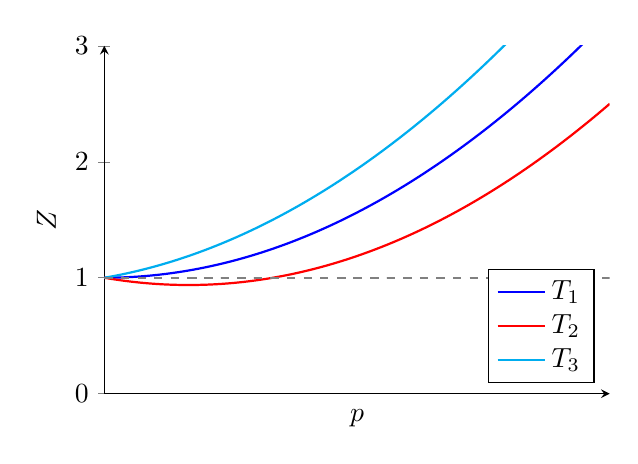
\begin{tikzpicture}
    \begin{axis}[
        width = 8cm,
        height = 6cm,
        legend pos = south east,
        xlabel = {$p$},
        ylabel = {$Z$},
        axis lines = left,
        ymin = 0,
        ymax = 3,
        xtick = \empty,
        domain = 0:3,
        samples = 400
    ]
    \addplot [thick, blue] {0.25*x^2+1};
    \addplot [thick, red] {0.25*(x-0.5)^2+15/16};
    \addplot [thick, cyan] {0.25*(x+0.5)^2+15/16};
    \addplot [thick, dashed, gray] {1};
    \legend {$T_1$,$T_2$,$T_3$}
    \end{axis}
\end{tikzpicture}
\end{document}
\end{figure}\\
\indent 在某个特定的温度(即图中的$T_1$)下,当压力在$p=0$附近的一定范围内,$Z$的变化都不大,即满足
\[\left(\dfrac{\p Z}{\p p}\right)_{T,p\to0}=0\]
时,在这一范围内用理想气体状态方程描述实际气体的偏差都是十分小的.%
这时的$Z-p$曲线满足$p=0$时$Z$对$p$的偏导数为$0$.对这样的温度$T_1$,我们做如下定义.
\begin{definition}[1C.1.2 实际气体的波义耳温度]
    定义实际气体的\tbf{波义耳温度}$T_B$为使得
    \[\left(\dfrac{\p\left(p\Vm\right)}{\p p}\right)_{T_B,p\to0}=0\]
    的温度.
\end{definition}
当温度低于$T_B$时,$\left(\dfrac{\p\left(p\Vm\right)}{\p p}\right)_{T_B,p\to0}<0$.根据导数的知识,存在一段压强范围使得$Z<1$,即气体容易被压缩而液化.%
反之,当温度高于$T_B$时,恒有$Z>1$,气体难以被压缩而液化.%
\vspace{4pt}\\
\Part{实际气体的$p-V$图}
\indent 除了$Z-p$图之外,我们还有一种描述实际气体行为的图像,即定温条件下的$p-\Vm$图.我们给出$\text{CO}_2$在各个温度下的$p-\Vm$图以供参考(原谅笔者懒得自己画于是找了一张图).
\begin{figure}[H]
    \centering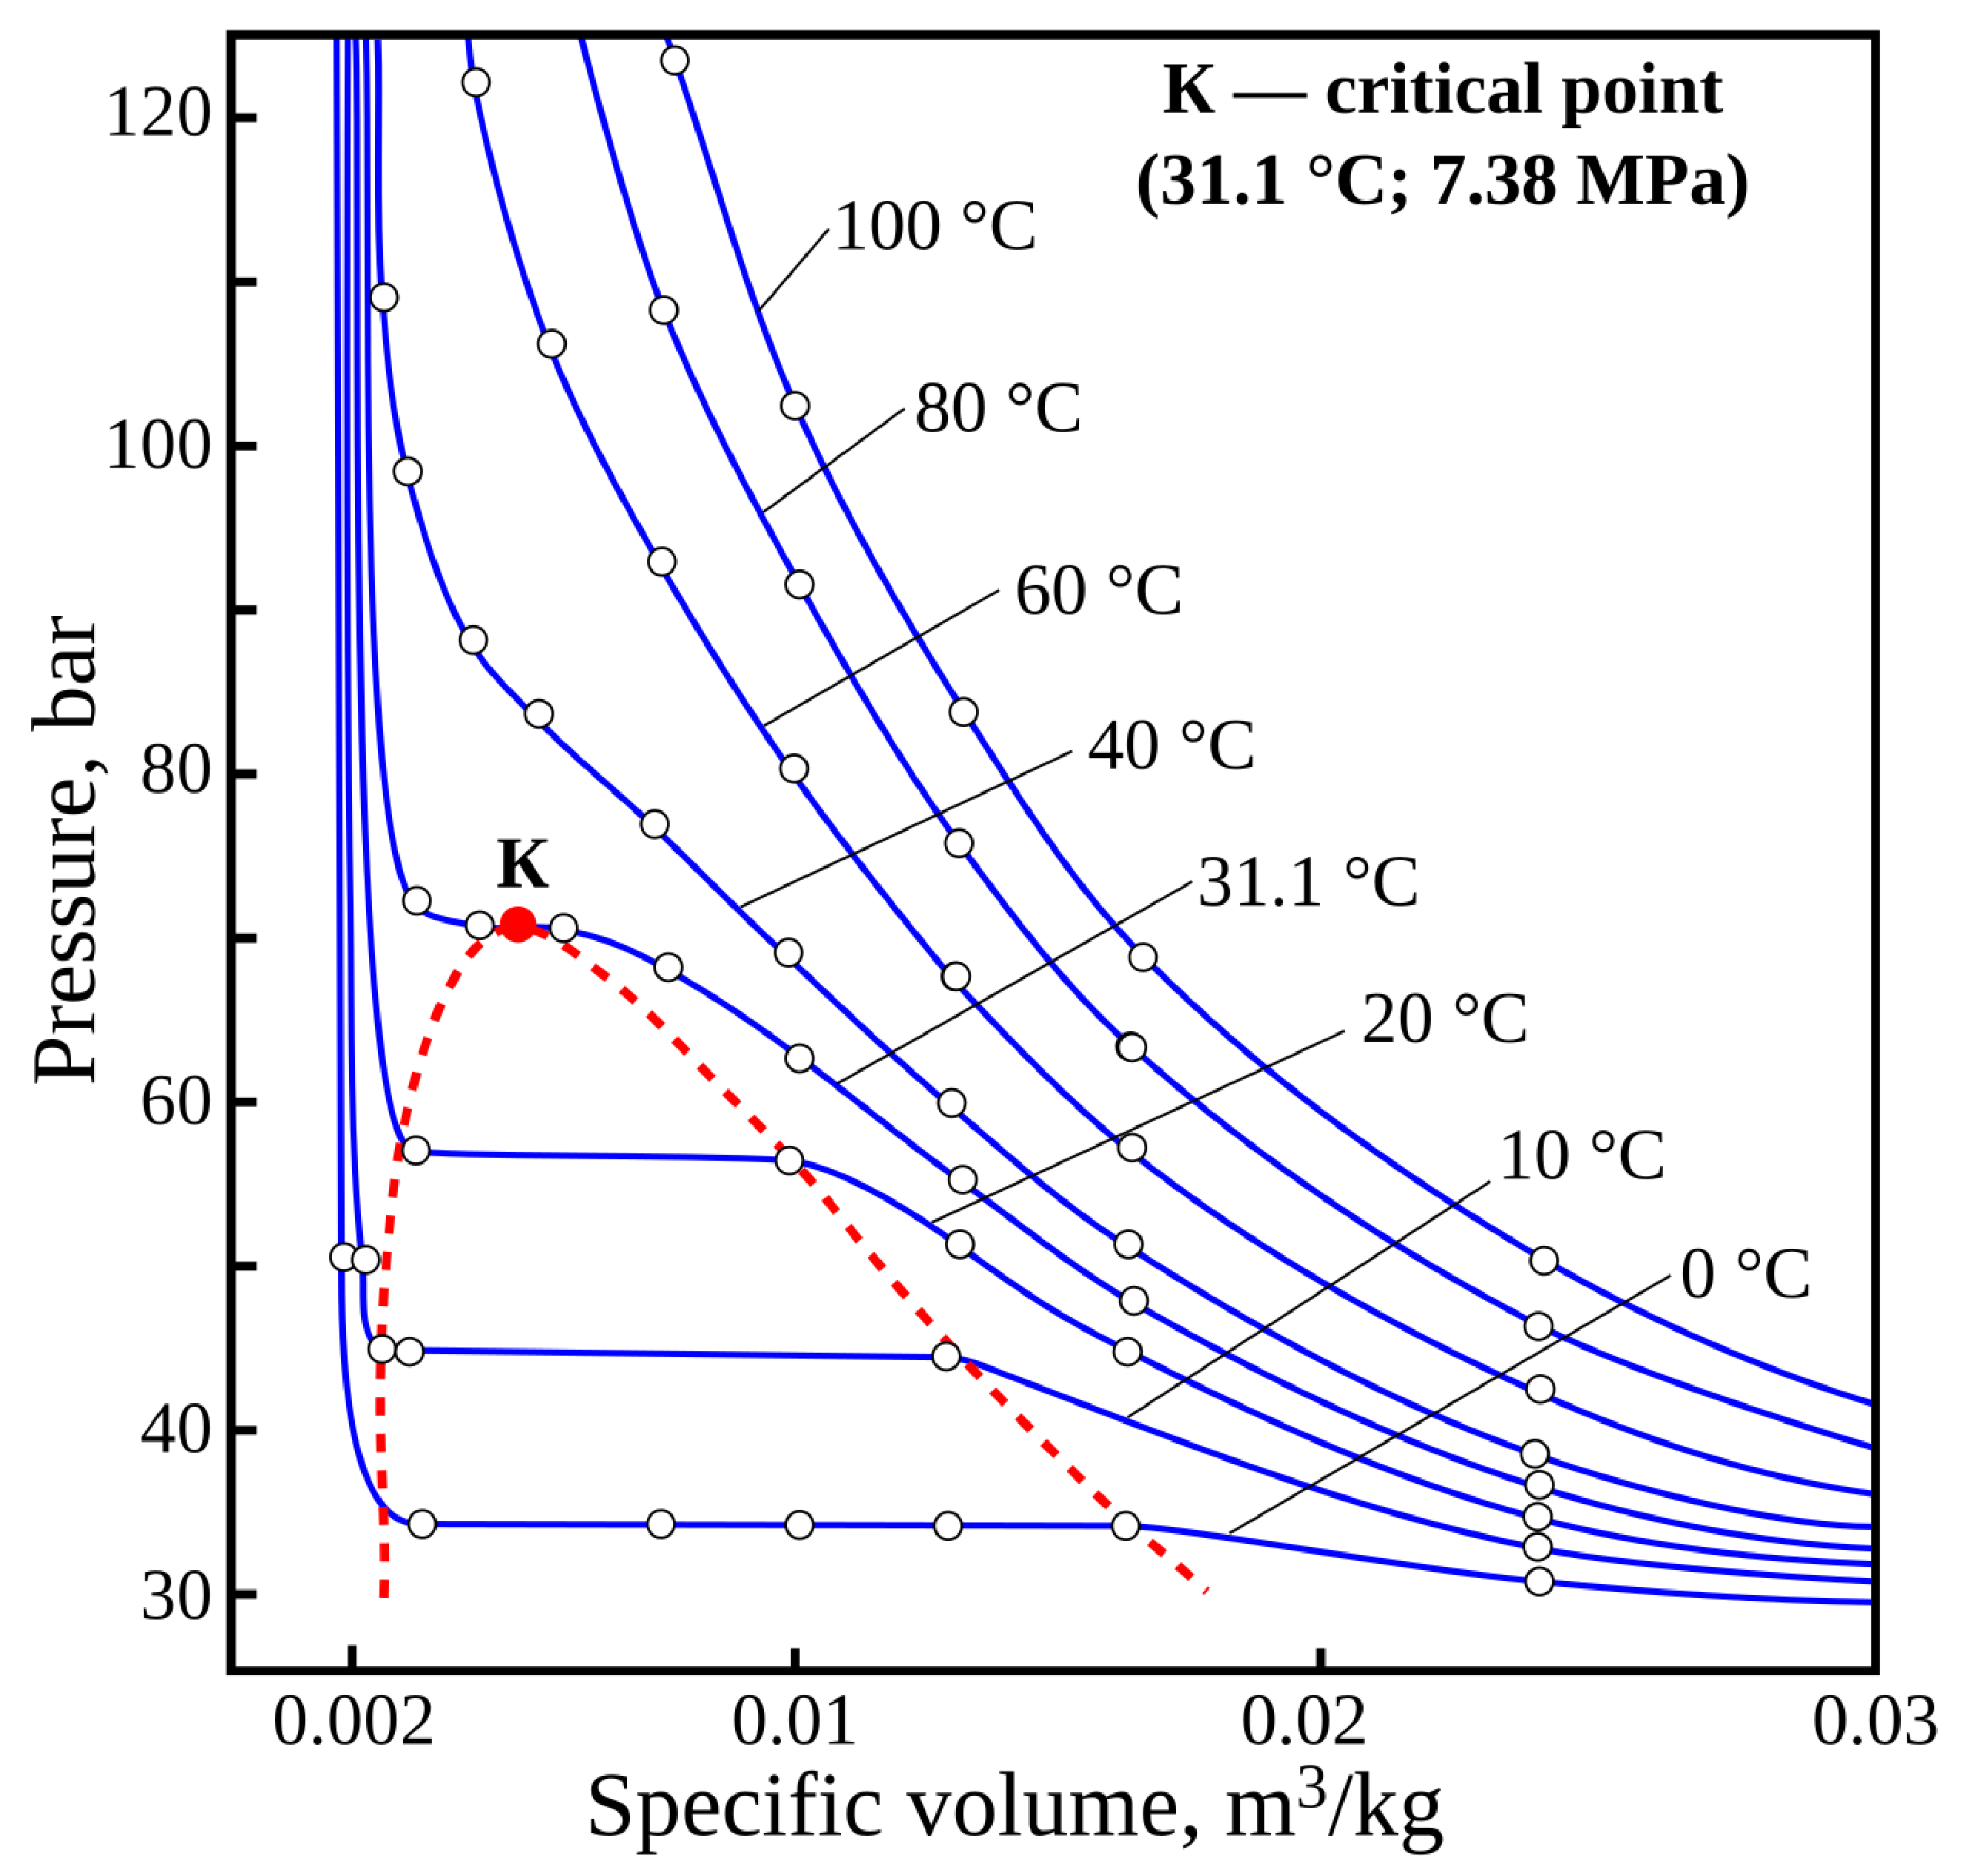
\includegraphics[scale=0.2]{picture/realCO2p-V.eps}
\end{figure}
上图中的曲线大致可以分为三类.\\
\indent 在较低的温度下,曲线大致可以分为三段.当$\Vm$较大时,曲线符合气体的一般性质,即体积减小(压缩)时压力增大.%
然而,中间出现了一段水平线,表明此时压缩并不改变体系的压力.由此可以想见,气体在此过程中发生了液化,这条线上$\Vm$的减小表示液相占比的增多.%
最后一段时,已经完全是液体,压力线陡然上升,表示液体不易压缩.\\
\indent 在较高的温度下,曲线大致符合等轴双曲线的形状,即$pV=C$,表示此时$\text{CO}_2$的性质与理想气体差别不大.\\
\indent 我们注意到在这些曲线中有这样特殊的一条:等温线的水平部分缩成一点,在此出现\tbf{拐点}.
\begin{hint}
    曲线的\tbf{拐点}的严格定义是曲线凹凸性发生改变的点.对于一个函数$f(x)$,如果点$\left(x_0,f\left(x_0\right)\right)$是此函数(图像)的拐点,那么我们有%
    $f'\left(x_0\right)=f''\left(x_0\right)=0\neq f'''\left(x_0\right)$.
\end{hint}
你可以注意到,在这条线上方,不再出现表示气液共存的水平线.这代表一个简单的事实:在此曲线对应的温度之上,你无论如何操作都不再能得到液体.%
反之,在此温度之下,总存在气液共存的状态.我们给这一特殊的温度及其状态做如下定义.
\begin{definition}[1C.1.3 临界态与超临界态]
    \tbf{临界态}是指纯物质的气,液两相平衡共存的极限状态.此时的温度为\tbf{临界温度}$T_\text c$,%
    此时的压力为\tbf{临界压力}$p_\text c$,体积为\tbf{临界体积}$V_\text c$,统称为\tbf{临界常数}.该状态对应的等温线为\tbf{临界等温线}.\\
    温度高于临界温度,压力高于临界压力的状态即为\tbf{超临界态}.
\end{definition}
在临界态下,气-液两相的一切差别都消失了,比体积相同,表面张力为零,汽化热为零,因而气液两相的界面也将消失.%
在超临界态下,物质兼具气体和液体的性质,在工业上也有一定的应用(例如用超临界$\text{CO}_2$萃取咖啡因).\\
\indent 我们对上述图中的区域也做一些描述.高于临界等温线的区域为单相区域,如果此时压力还高于临界压力,那么物质为超临界态,否则为气态;%
温度低于临界温度时,中间的帽形区域为气液两相共存的区域,帽形区域的边界与临界等温线所夹区域的左半部分为纯液相,右半部分为纯气相.\\
\indent 可以看出,当压力足够低或温度足够高时,气体总是无法液化,说明分子间作用力并不显著.此时的气体接近于理想气体.%
\vspace{12pt}\\
\Section{1C.2 维里(位力)方程}
\indent 对于现实中的问题,我们很难用纯理论化的方式对其进行量化.迄今以来,以及你以后看到的许多公式都只存在纸面上,尽管再精密,都和现实世界有一定的差距.%
实际气体的状态方程就是这样的问题.不过,我们还有一计:用足够多的参数拟合.\\
\indent 维里方程,又称为维里展开(virial expansion,此处的维里和位力都是音译),由Kammerlingh Onnes提出,就是这样的一个用于拟合实际气体状态方程的方法.
\begin{theorem}[1C.2 维里方程]
    在一定的温度下,压缩因子$Z$应当是$p$或者$\dfrac{1}{V_\text m}$的函数.\\
    将$Z$对$p$做级数展开,则有
    \[Z=1+B'p+C'p^2+\cdots\]
    或者更常见地,对$\dfrac{1}{V_\text m}$做级数展开
    \[Z=1+\dfrac{B}{\Vm}+\dfrac{C}{\Vm^2}+\cdots\]
    系数$B',C',\cdots$或$B,C,\cdots$被称为第二,第三,$\cdots$\tbf{维里系数},它们是关于温度的函数.\\
    维里系数可以通过测定实际气体的$p-\Vm-T$数据后拟合得到.
\end{theorem}
在这里,我们需要做一些额外的说明.我们所说的压力$p\to0$时,实际气体符合理想气体状态方程,\tbf{并非}符合理想气体的所有性质.%
例如,理想气体的压缩因子$Z$不论何时都等于$1$,因此对$p$的变化率$\dfrac{\di Z}{\di p}=0$.%
然而,对于符合维里方程(我们采取第一种形式)的实际气体,则有
\[\dfrac{\di Z}{\di p}=B'+2C'p+\cdots\]
当$p\to0$时有$\dfrac{\di Z}{\di p}=B'$.因此,变化率这一性质不一定与理想气体相符.%
然而,当上式中$B'=0$时,我们有
\[\left(\dfrac{\p\left(p\Vm\right)}{\p p}\right)_{T_B,p\to0}=\left(\dfrac{\di Z}{\di p}\right)_{p\to0}=B'=0\]
此时对应的温度即为波义耳温度.在波义耳温度下,气体符合$pV\approx nRT$的压力范围比其它温度下更宽.\\
\indent 维里方程在实际生产过程中应用广泛(只要你的数据测得够多够准,你就可以得到足够精度的方程),%
并且无需对底层的热力学有了解.它甚至还可以用于液体和固体的状态方程.所谓参数够多,你就是造物主.%
\vspace{12pt}\\
\Section{1C.3 van der Waals方程}
\Part{van der Waals方程及其物理意义}
\indent 在所有描述实际气体的状态方程中,van der Waals(范德华)方程是最有名的.不仅是因为它与实验数据符合的相当好,%
还因它对理想气体状态方程进行了有物理意义的修正,而非简单的拟合(比如那些费尽心思凑出符合实验数据的公式的可怜的科研人员们).%
\begin{theorem}[1C.3.1 van der Waals 方程]
    我们有
    \[\left(p+\dfrac{a}{\Vm^2}\right)\left(\Vm-b\right)=RT\]
    其中$a,b$为修正项,其物理意义将在接下来叙述.
\end{theorem}
\begin{derivation}
    我们来讨论如何得到这两个修正项.\\
    理想气体状态方程$p\Vm=RT$中的$\Vm$应当指气体分子能自由活动的体积.%
    现实世界中,我们不能忽略分子自身的体积,因此$\Vm$需要减去体积修正项$b$.\\
    我们仍然拿出我们的边长为$l$的正方体容器,并且向其中一个一个地加入半径为$r$的球体分子.\\
    计算这些气体分子能自由活动的范围时,我们仍然把它们抽象成质点,但是任意两个质点之间的间距不能小于$2r$.\\
    放入第一个分子$X_1$,它与所有壁都至少应保持$r$的距离(后面的分子也一样),因此它能自由活动的体积为
    \[V_{1,\text{free}}=\left(l-2r\right)^3\]
    第二个分子$X_2$除了与器壁保持不小于$r$的距离之外,还要求不能进入以第一个分子为球心,半径为$2r$的球内.因此$X_2$能自由活动的体积为
    \[V_{2,\text{free}}=\left(l-2r\right)^3-\dfrac43\pi\left(2r\right)^3\]
    依次类推,放入第$N$个分子$X_N$后,它能自由活动的体积为
    \[V_{N,\text{free}}=\left(l-2r\right)^3-(N-1)\cdot\dfrac43\pi\left(2r\right)^3\]
    平均来说,每个分子能自由活动的体积为
    \[\begin{aligned}
        \overline{V_{\text{free}}}
        &= \dfrac{1}{N}\sum_{i=1}^{N}V_{i,\text{free}} \\
        &= \dfrac{1}{N}\sum_{i=1}^{N}\left(\left(l-2r\right)^3-(i-1)\cdot\dfrac43\pi\left(2r\right)^3\right) \\
        &= (l-2r)^2-\dfrac1N\cdot\dfrac{N(N-1)}{2}\cdot\dfrac{32}{3}\pi r^3 \\
        &\xlongequal{N\gg 1,l\gg r}V-N\cdot\dfrac{16}{3}\pi r^3
    \end{aligned}\]
    按体积修正量的定义,此容器体积应为$\Vm$,含有$\NA$个分子.因此,体积修正项为
    \[b=4\NA\cdot\dfrac43\pi r^3\]
    即体积修正项为$1\text{mol}$分子体积总和的四倍.\\
    气体分子之间的作用力也是不可忽略的.当气体分子靠近容器壁时,在容器壁一侧的分子数目少,对其作用力小;在远离容器壁一侧的分子数目多,对其作用力大.%
    总体来说,气体分子在靠近器壁时会被其余分子向后拉,导致实际压力小于理论压力.\\
    我们把这一差值称为\tbf{内压力}$p_\text i$.既然内压力是由于气体分子之间的相互吸引造成的,这一作用应当同时造成气体碰撞频率和碰撞时的动量的同时减小.%
    而这两个量的减少各自都应正比于分子分布的密度$\rho=\dfrac NV$.因此(直觉地)可以得出,$p_\text i$应当与$\rho^2$成正比,又因为$\rho=\dfrac{\NA}{\Vm}$,于是
    \[p_\text i\varpropto\dfrac{1}{\Vm^2}\text{\ \ \ 或\ \ \ }p_\text i=\dfrac{a}{\Vm^2}\]
    上式中的$a$就是分子间引力的校正项.
\end{derivation}
\Part{van der Waals气体的$p-V$图}
\indent 虽然van der Waals方程并不是一个完全准确的方程,但由于其中的修正都是有比较明确的物理意义的,因此是我们研究实际气体行为的一个重要工具.%
下图给出了将$\text{CO}_2$当作van der Waals气体处理时,在各自温度下得到的$p-\Vm$图.
\begin{figure}[H]
    \centering\documentclass{standalone}
\usepackage{PhysicalChemistryNote}
\begin{document}
\begin{tikzpicture}
    \begin{axis}[
        width = 8cm,
        height = 8cm,
        legend pos = north east,
        xlabel = {$\Vm/\left(\text{cm}^{3}\cdot\text{mol}^{-1}\right)$},
        ylabel = {$p/10^3\text{kPa}$},
        axis lines = left,
        ymin = 5,
        ymax = 10,
        domain = 50:300,
        samples = 400
    ]
    \addplot [thick, blue, domain = 55:300] {2395.68/(x-42.7)-361000/(x^2)};
    \addplot [thick, red] {2493.31/(x-42.7)-361000/(x^2)};
    \addplot [thick, cyan] {2520.39/(x-42.7)-361000/(x^2)};
    \addplot [thick, violet] {2603.53/(x-42.7)-361000/(x^2)};
    \legend {$T=15\tccentigrade$,$T=26.7\tccentigrade$,$T=30\tccentigrade$,$T=40\tccentigrade$}
    \end{axis}
\end{tikzpicture}
\end{document}
\end{figure}
\indent 我们似乎可以注意到,当温度低于某个温度时(例如图中的$15\tccentigrade$),$\text{CO}_2$似乎在某一段上出现了%
压力和体积同时增大的状况.想想这个诡异的情况吧!当你把这气体放在带活塞的容器内并用力压它时,竟然会出现体积增大的现象.这是怎么一回事呢?\\
\indent 事实上,如果你还记得我们在\tbf{1C.1}中给出的实际情况下$\text{CO}_2$的$p-\Vm$图,就会发现这诡异的一段(和它左右的一小部分)实际上是代表气体发生液化的气液共存线,就像下面这样.
\begin{figure}[H]
    \centering\documentclass{standalone}
\usepackage{PhysicalChemistryNote}
\begin{document}
\begin{tikzpicture}
    \begin{axis}[
        width = 8cm,
        height = 8cm,
        legend pos = north east,
        xlabel = {$\Vm/\left(\text{cm}^{3}\cdot\text{mol}^{-1}\right)$},
        ylabel = {$p/10^3\text{kPa}$},
        axis lines = left,
        ymin = 5,
        ymax = 10,
        samples = 400
    ]
    \addplot+ [black, only marks, point meta = explicit symbolic, nodes near coords, clip = false]
        table [meta=name] {
		x y name
        89.533 6.1196 $\ \ A$
		102.31 5.701 $B$
        166.878 6.3292 $C$
        211.83 6.1196 $D$
		};
    \addplot [thick, blue, domain = 50:89.53] {2395.68/(x-42.7)-361000/(x^2)};
    \addplot [thick, blue, domain = 211.83:300] {2395.68/(x-42.7)-361000/(x^2)};
    \addplot [thick, dashed, gray, domain = 89.53:211.83] {2395.68/(x-42.7)-361000/(x^2)};
    \addplot [thick, blue, domain = 89.2:212] {6.1196};
    \legend {,$T=15\tccentigrade$};
    \end{axis}
\end{tikzpicture}
\end{document}
\end{figure}
\indent 这一段不太符合事实的曲线段$ABCD$,我们定义为\tbf{范德华环(van der Waals loops)}.替代范德华环的线段$AD$将曲线分为面积相等的两个部分,%
这一替代称为\tbf{麦克斯韦构造(Maxwell construction)}.
\begin{hint}
    关于Maxwell构造的物理意义,我们将在\tbf{Chapter 4}中讲到实际气体的相变时再讨论.
\end{hint}
虽然$BC$段的上升是没有实际意义的(就像我们前面所说的那样),但在特定条件下,人们仍然复现了$AB$段和$CD$段的实验结果.\\
\indent 将气体在没有尘埃和电荷的空间中加压,则气体会由于缺乏凝结核而成为\tbf{过饱和蒸汽},即图中的$CD$段.如果向体系引入带电粒子,%
那么气体将迅速凝结为液体,回到$AD$这条气液平衡线上.Wilson云雾室就是利用了气体的这一性质,将带电粒子射入过饱和蒸汽中,当粒子与蒸汽分子碰撞后,%
蒸气就将以这些被碰撞的分子为中心液化,形成一连串小液滴,从而反映其轨迹.\\
\indent 同样地,将纯的液体自$A$点等温减压,由于缺少气化中心\footnote{以后我们会知道,由于表面张力的缘故,纯液相中较难出现气泡.}%
液体会下降到$B$点而不气化,成为\tbf{过热液体}.%
稍有扰动,液体就将发生剧烈气化,即\tbf{暴沸}现象.如果在实验或实际生产中出现这一现象,会造成巨大安全隐患. %
锅炉内反复煮沸的水,微波炉内加热的牛奶等等都可能发生暴沸.\\
\indent 我们由分析van der Waals方程得到了两种非平衡态的体系,即
\begin{definition}[1C.3.2 过饱和蒸汽]
    \tbf{过饱和蒸汽}是指蒸汽超过该温度下的饱和压力而不发生相变的现象.\\
    从饱和蒸汽表来看,过饱和蒸汽的压力所对应的饱和温度高于目前本身的温度,所以过饱和蒸汽也叫做\tbf{过冷蒸汽}.
\end{definition}
\begin{definition}[1C.3.3 过热液体与暴沸]
    \tbf{过热}是指液体被加热到沸点以上的温度而不沸腾的现象,这样的液体称为\tbf{过热液体}.\\
    \tbf{暴沸}是指过热液体突然剧烈沸腾的现象,通常在过热液体接触气泡或杂质时发生.
\end{definition}
这说明van der Waals方程对实际气体的某些性质具有较好的符合性质.\vspace{4pt}\\
\Part{van der Waals气体的临界常数}
\indent 对van der Waals气体的数学处理也是丰富而具有深刻的物理意义的,我们将在接下来给出一些例子.例如,我们可以求算van der Waals气体的临界温度$T_\text c$.
\begin{derivation}
    我们在\tbf{1C.1.3}中已经知道临界温度$T_\text c$下,曲线
    \[p=\dfrac{RT_\text c}{\Vm-b}-\dfrac{a}{\Vm^2}\]
    有拐点,于是存在$\Vm$使得
    \[\left\{\begin{array}{l}
        \dfrac{\di p}{\di\Vm}=\dfrac{2a}{\Vm^3}-\dfrac{RT_\text c}{\left(\Vm-b\right)^2}=0 \\
        \dfrac{\di^2p}{\di\Vm^2}=\dfrac{2RT_\text c}{\left(\Vm-b\right)^3}-\dfrac{6a}{\Vm^4}=0
    \end{array}\right.\]
    于是
    \[\dfrac{\left(\Vm-b\right)^2}{\Vm^3}=\dfrac{RT_\text c}{2a}\ \ \ \ \ \dfrac{\left(\Vm-b\right)^3}{\Vm^4}=\dfrac{RT_\text c}{3a}\]
    于是
    \[\dfrac{\left(\Vm-b\right)^2}{\Vm^3}=\dfrac32\cdot\dfrac{\left(\Vm-b\right)^3}{\Vm^4}\]
    于是
    \[\Vm=3b\]
    回代可得
    \[T_\text c=\dfrac{8a}{27Rb}\ \ \ \ \ p=\dfrac{a}{27b^2}\]

\end{derivation}
于是我们有
\begin{theorem}[1C.3.4 van der Waals气体的临界态]
    van der Waals气体的临界常数为
    \[T_\text c=\dfrac{8a}{27Rb}\ \ \ \ \ V_{\text m,\text c}=3b\ \ \ \ \ p_\text c=\dfrac{a}{27b^2}\]

\end{theorem}
因此,可以通过测量$T_\text c$和$p_\text c$来得到$a,b$($V_{\text m,\text c}$不易测准,故不采用),即
\[a=\dfrac{27}{64}\dfrac{R^2T_\text c^2}{p_\text c}\ \ \ \ \ b=\dfrac{RT_\text c}{8p_\text c}\]
\indent 通过适当的化简,我们还可以得到一个与$a,b$无关的式子,即
\[\dfrac{RT_\text c}{p_\text cV_{\text m,\text c}}=\dfrac83\]
所有van der Waals气体均应当满足此等式.不过,实际测量表明,只有He,$\text H_2$等难以液化的气体才符合上述等式,可见van der Waals方程在极端条件下仍然有局限性.\vspace{4pt}\\
\Part{对比状态定律}
\indent 科学上研究不同物质特性的一种通用的方法是为它们选择一个同类的物理性质,并以此为基础设置一个相对标度.%
气体的临界常数就是一个很好的标定方法(这时的气体有诸多相似之处,我们已经在前面叙述过).因此,我们可以以此为基准建立一套标度体系.
\begin{definition}[1C.3.5 对比变量]
    将气体的各状态函数与临界常数做比得到的无量纲量称作气体的\tbf{对比变量},即
    \[V_\text r=\beta=\dfrac{\Vm}{V_{\text m,\text c}}\ \ \ \ \ p_\text r=\pi=\dfrac{p}{p_\text c}\ \ \ \ \ T_\text r=\tau=\dfrac{T}{T_\text c}\]
    其中$V_\text r,p_\text r,T_\text r$和$\beta,\pi,\tau$为不同出处的记法.$\beta,\pi,\tau$分别称作\tbf{对比体积},\tbf{对比压力}和\tbf{对比温度}.
\end{definition}
\tbf{1C.3.4}的推导中已经将$a,b$和$R$用临界常数表出,因此van der Waals方程可以写作用临界常数表达的形式.%
那么这是否意味着对比变量之间也有类似于状态方程的等量关系呢?答案是肯定的.
\begin{derivation}
将我们在推导\tbf{1C.3.4}时求算的$a,b$和$R$代入\tbf{1C.3.1}可得
\[\left(p+\dfrac{3p_\text cV_{\text m,\text c}^2}{\Vm^2}\right)\left(\Vm-\dfrac{V_{\text m,\text c}}{3}\right)=\dfrac83\dfrac{p_\text cV_{\text m,\text c}}{T_\text c}T\]
两边同时除以$p_cV_{\text m,\text c}$可得
\[\left(\dfrac{p}{p_\text c}+\dfrac{3V_{\text m,\text c}^2}{\Vm^2}\right)\left(\dfrac{\Vm}{V_{\text m,\text c}}-\dfrac{1}{3}\right)=\dfrac83\dfrac{T}{T_\text c}\]
即
\[\left(\pi+\dfrac{3}{\beta^2}\right)\left(3\beta-1\right)=8\tau\]

\end{derivation}
\begin{theorem}[1C.3.6 van der Waals气体的对比状态定律]
    任何van der Waals气体都满足
    \[\left(\pi+\dfrac{3}{\beta^2}\right)\left(3\beta-1\right)=8\tau\]
    
\end{theorem}
事实上,我们有
\begin{theorem}[1C.3.7 对比状态定律]
    在相同的对比体积和对比温度之下,不同的真实气体具有相同的对比压力,这一状态被称为\tbf{对比状态}.
\end{theorem}
对比状态定律对结构相近的分子符合地较好.在相同的对比状态下,这些物质的诸多物理性质(例如折射率,黏度等)具有简单的关系.%
这一定律很好地表现了宏观性质与微观结构的相关性.\\
\indent “对比状态定律确实可以看作van der Waals方程最有用的副产品.”Guggenhum如是说.
\end{document}
\end{document}